%%%% Better Poster latex template example v1.0 (2019/04/04)
%%%% GNU General Public License v3.0
%%%% Rafael Bailo
%%%% https://github.com/rafaelbailo/betterposter-latex-template
%%%% 
%%%% Original design from Mike Morrison
%%%% https://twitter.com/mikemorrison

\documentclass[a0paper,fleqn]{src/betterposter}

\begin{document}	
\betterposter{
%%%%%%%% MAIN COLUMN

\maincolumn{
%%%% Main space

\textbf{From code to deployment}\\
\fontsize{75}{77}\selectfont % Set the font size to 12pt with a baseline skip of 14pt

Pull-request workflow\\[1.5cm]
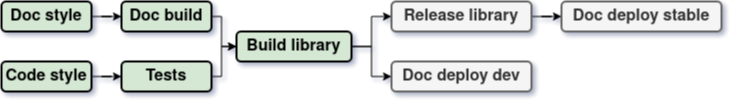
\includegraphics[width=\textwidth]{img/ci_cd/ci_cd_pr}\\

Main branch workflow\\[1.5cm]
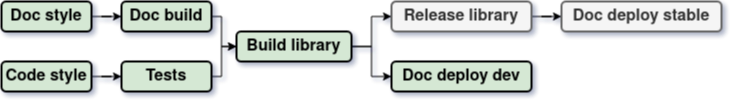
\includegraphics[width=\textwidth]{img/ci_cd/ci_cd_main}\\

Release workflow\\[1.5cm]
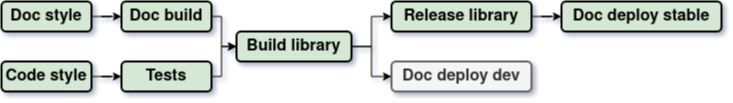
\includegraphics[width=\textwidth]{img/ci_cd/ci_cd_release}\\

\fontsize{85}{87}\selectfont
Use ansys/actions@v4\\[1cm]

\vspace{-18cm}

}{
%%%% Bottom space

%% QR code
\qrcode{img/ci_cd/qrcode.png}{img/example/smartphoneBlack}{
\textbf{Visit https:\slash \slash actions.docs.ansys.com for more information}
}
% Smartphone icon
% Author: Freepik
% Retrieved from: https://www.flaticon.com/free-icon/smartphone_65680

%% Compact QR code (comment the previous command and uncomment this one to switch)
%\compactqrcode{img/example/qrcode}{
%\textbf{Take a picture} to
%\\download the full paper
%}

}

}{
%%%%%%%% LEFT COLUMN

\title{CI\slash CD pipelines for scientists}
\author{Jorge Martinez}
\institution{Ansys}

\section{
\includegraphics[height=\fontcharht\font`\S]{img/example/slash.png} Introduction}
CI/CD is used for empowering software development through automated integration
and deployment, revolutionizing efficiency and reliability in the software
delivery lifecycle.


\section{
\includegraphics[height=\fontcharht\font`\S]{img/example/slash.png}Code style}
Enforcing consistency and code quality through automated analysis, ensuring clean and maintainable software development practices.

\section{
\includegraphics[height=\fontcharht\font`\S]{img/example/slash.png} Fundamental Theorem\\of Calculus}
If $f$ is continuous on the closed interval $[a,b]$ and $F$ is the indefinite integral of $f$ on $[a,b]$, then
\begin{equation}
\int_a^b f(x)\,\mathrm{d}x = F(b)-F(a).
\end{equation}

\section{
\includegraphics[height=\fontcharht\font`\S]{img/example/slash.png} Conclusion}
This is a great poster format!

%% This fills the space between the content and the logo
\vfill

%% Institution logo

\includegraphics[width=\textwidth]{img/example/pyansys_dark}\\

}{
%%%%%%%% RIGHT COLUMN

Here you can add \textbf{supplementary material}. For instance, a new diagram:
\begin{center}
% Commutative diagram with edges passing under/over
% Author: Stefan Kottwitz, http://texblog.net/
% Retrieved from: http://www.texample.net/tikz/examples/commutative-diagram/
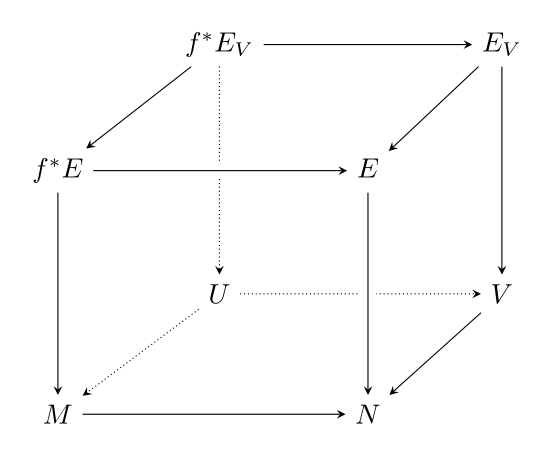
\includegraphics[width=\textwidth]{img/example/tikzexample2}
\end{center}

Some cute ducklings:
\begin{center}
% Picture of ducklings
% Author: Magda Ehlers, https://www.pexels.com/@magda-ehlers-pexels
% Retrieved from: https://www.pexels.com/photo/selective-focus-photo-of-flock-of-ducklings-perching-on-gray-concrete-pavement-1300355/
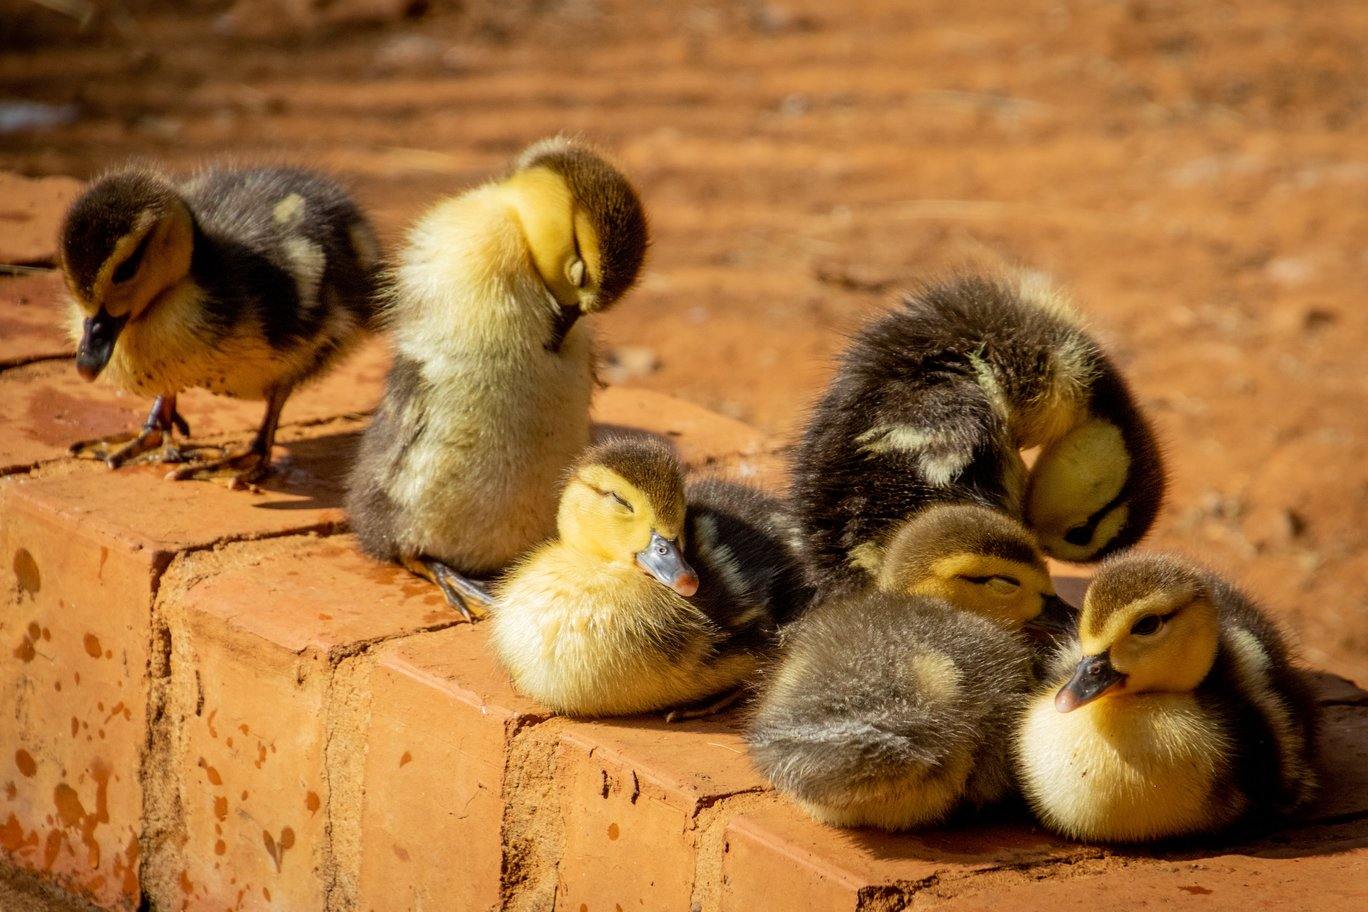
\includegraphics[width=\textwidth]{img/example/ducklings}
\end{center}
}
\end{document}
